\documentclass{article}
\usepackage[utf8]{inputenc}
\usepackage{preamble}
\usepackage{siunitx}
\usepackage{physics}
\newcommand{\vecS}{\boldsymbol{\vec{S}}}

\begin{document}

\begin{center}
   \LARGE{\textsc{MATH 271, Project}}\\
   \large{\textsc{Due December 18$^\textrm{th}$}}
\end{center}
\vspace{.5cm}

\section*{Due Date}
The assignment must be turned in via Canvas by Friday December 18$^\textrm{th}$, 2020, by 11:59PM mountain time.
\subsection*{Requirements}
\begin{itemize}
    \item You may work together, but you must submit your own individual work.
    \item You are to type out your work to this assignment using a program like Microsoft Word or \LaTeX. If you use a program like Microsoft Word, use the equation editor for any mathematical symbols you use. 
    \item Save your document as a PDF as only PDF files will be accepted. Make sure your formatting comes out correctly when you save as a PDF! Microsoft Word has a way of making this more challenging than it needs to be.
    \item For full credit, explain your work along the way and use consistent notation.  Though problems may not ask for much, a short and complete explanation is expected.
\end{itemize}


\section{Introduction}

\subsection{A brief about particle physics}

Spin is an intrinsic quantity that is associated to all elementary and composite particles.  Elementary particles are those that appear in the \boldblue{standard model of particle physics}. 

\begin{figure}[H]
    \centering
    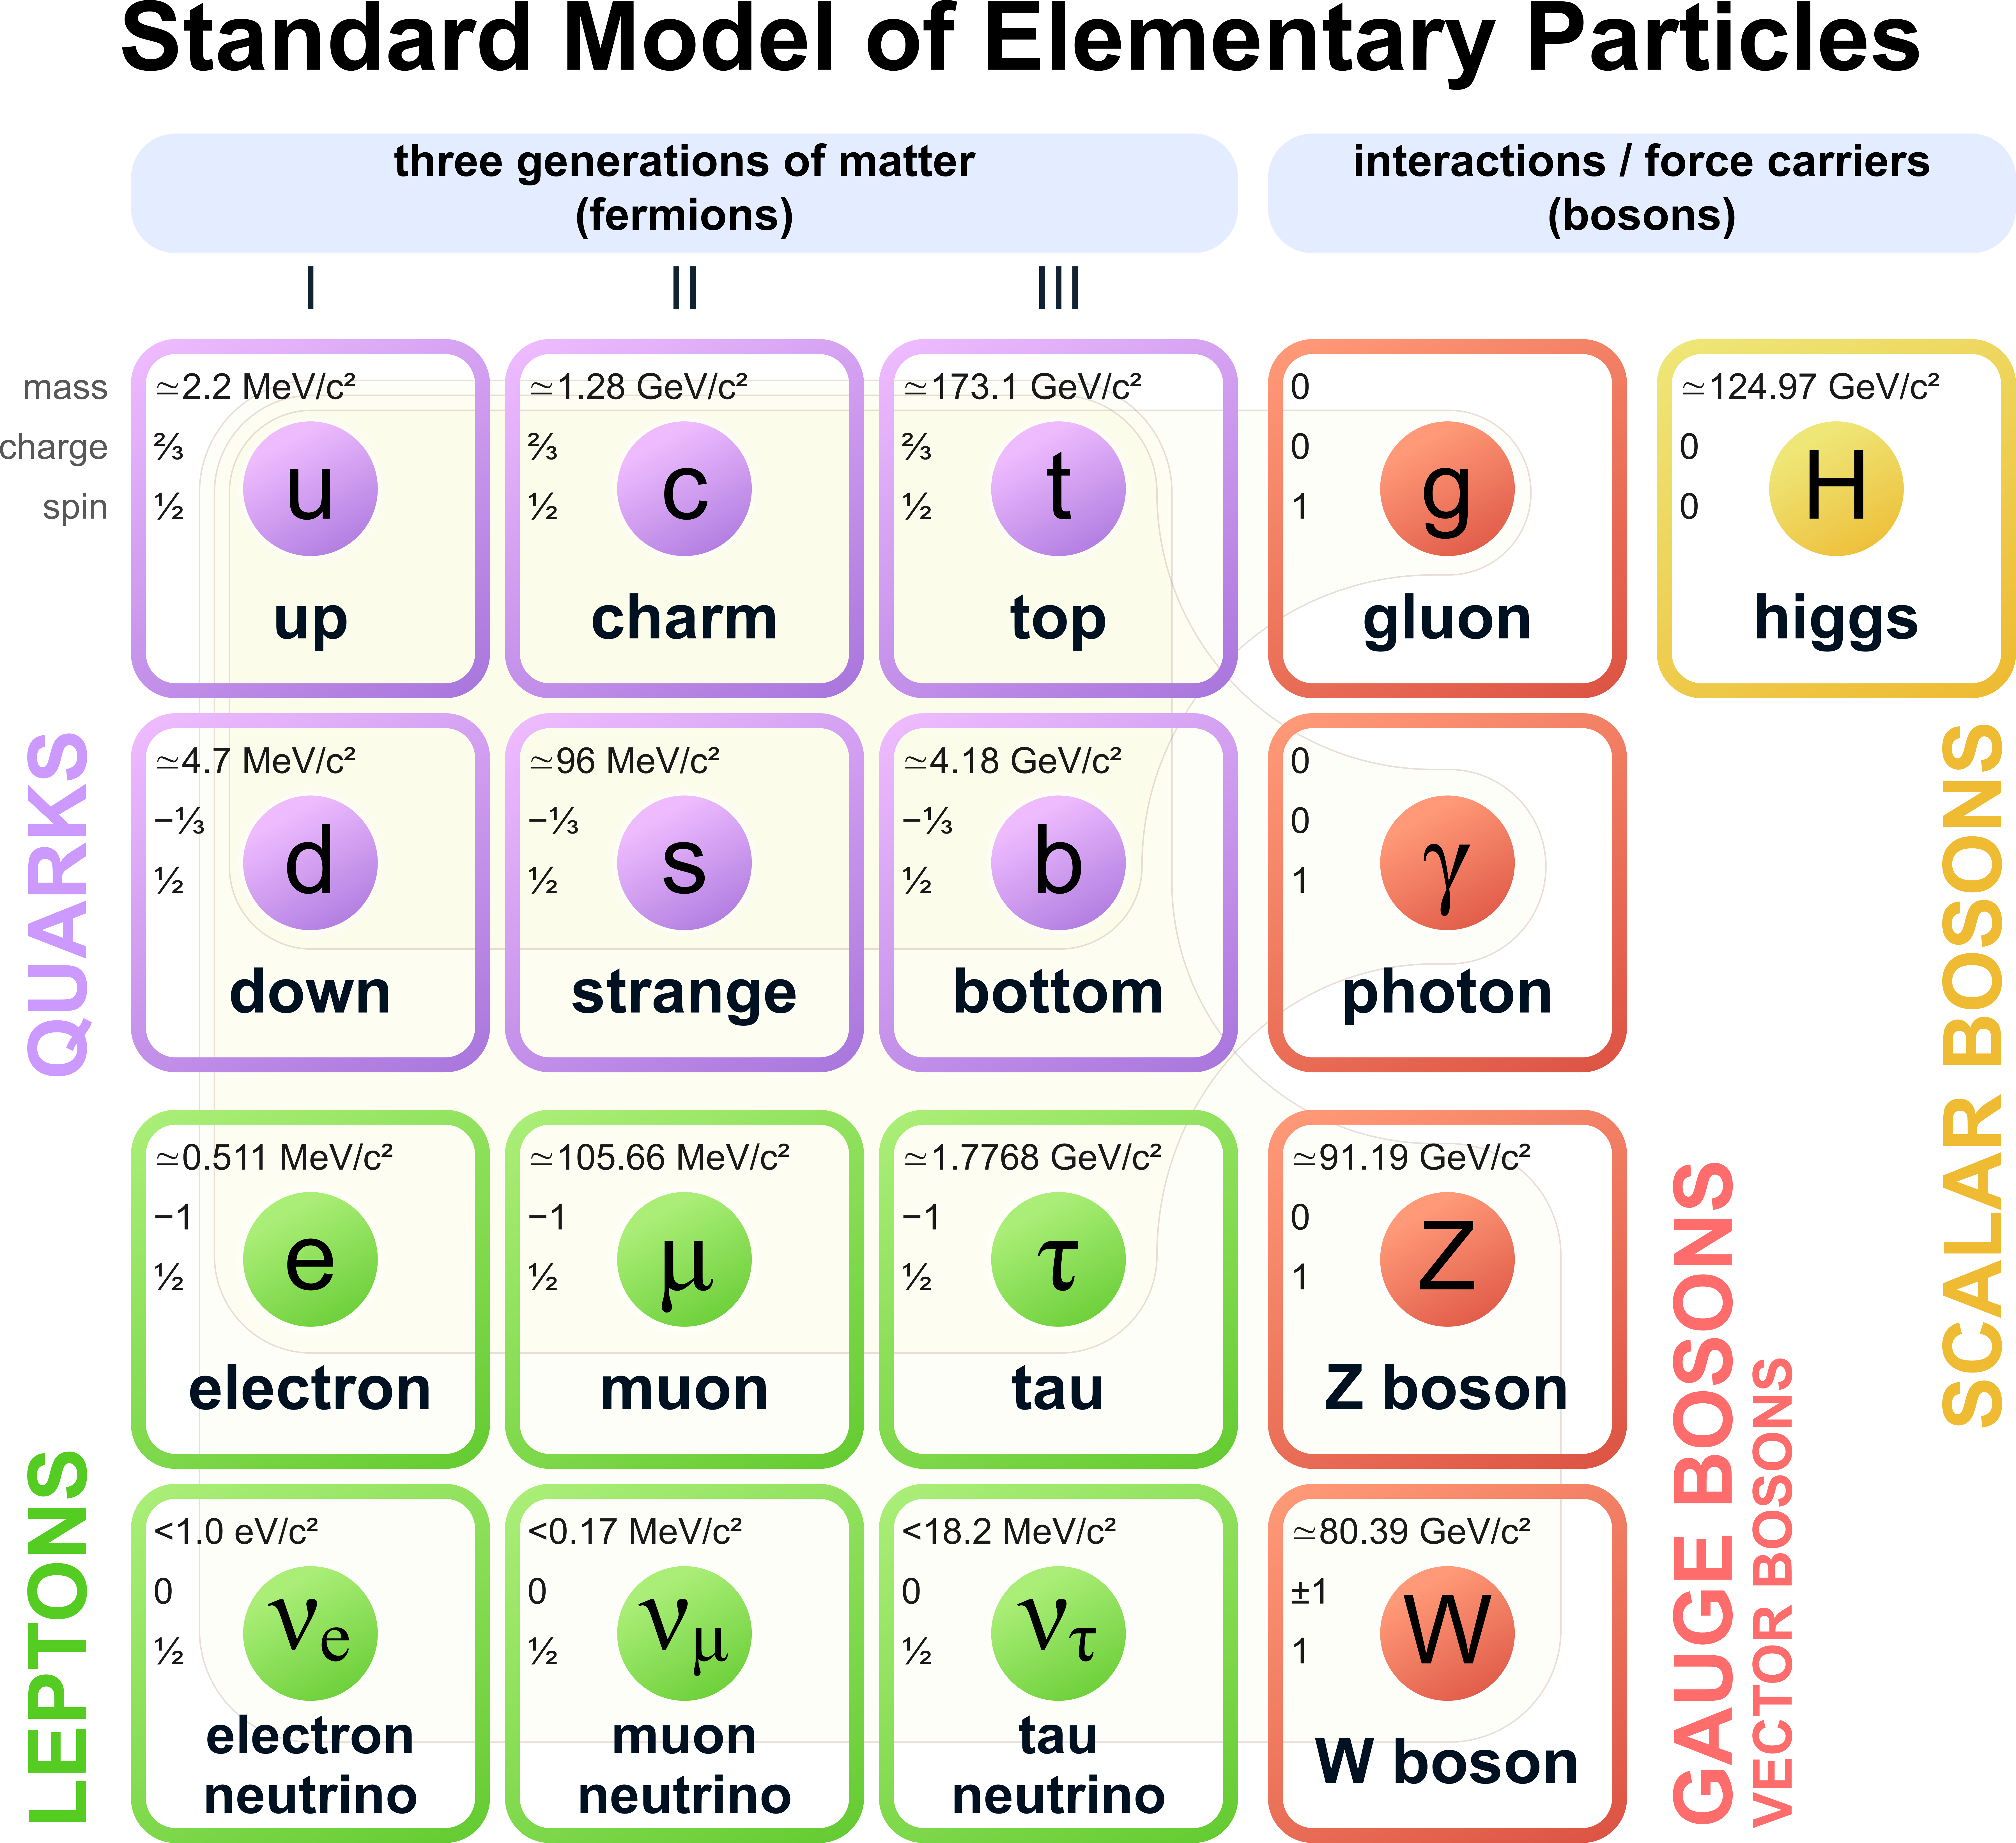
\includegraphics[width=.6\textwidth]{standard_model.png}
    \caption{The standard model.}
\end{figure}

From the particles in the standard model, we can create composite particles. Take note of the mass, charge, and spin for each one of these particles seen in Figure 1. Masses for these particles are given in units \si[per-mode=symbol]{\mega \electronvolt \per c \squared} where \si{\mega \electronvolt} is a megaelectronvolt and \si{c} is the speed of light in a vacuum. Charge is the quantity that couples these particles to the electromagnetic field.  In the sequel to 271, we will discuss electromagnetism and how stationary and moving charges create an electromagnetic field. 

For example, a neutron is composed of an up and two down quarks and a proton is composed of two up and a down quark. Other particles such as the photon and the electron we see by themselves throughout the universe. In fact, all leptons and all neutrinos can be readily observed passing through our atmosphere. One can even use muon's (a heavy cousin of the electron) to observe special relativity in action! 

\begin{problem}{Properties of neutrons and protons}{prob:1}
Given the make up of neutrons and protons mentioned in the previous paragraph, compute the following.
\begin{enumerate}[(a)]
    \item Add together the charges of constituent particles for the neutron and proton to show that you get the expected total charge of 0 and 1 respectively.
    \item Add together the masses of the constituent particles and compare that with the true mass of the neutron and proton. Is this mass the same?
\end{enumerate}
\end{problem}

One should find that while charges add, mass does not add.  As it turns out, much more takes place to give neutrons and protons their mass.  Similarly, one finds that the spin also does not add. Neutrons and protons are themselves particles that have a spin of 1/2. Neutrons are also not charged while protons do carry a charge of +1.  

\subsection{The Stern-Gerlach experiment}

Atoms are the building blocks for chemists. Every atom is a composite particle consisting of a nucleus containing a balance of neutrons and protons and electrons orbit around this dense positively charged nucleus.  In a neutral atom, we will always see the same number of electrons as protons and the number of neutrons may very (with certain isotopes being more common). In 272 we will discuss the structure of the hydrogen atom as it proves to be the simplest example since it can be modeled as a single charge with a single orbiting electron. The structure of atomic nuclei is far more involved.

If we have a charged particle with a nonzero radius associated to it, we can think of this particle as a loop with a current $\boldsymbol{\vec{I}}$. Basic electromagnetic theory tells us that a loop of current will create a magnetic field.

\begin{figure}[H]
    \centering
    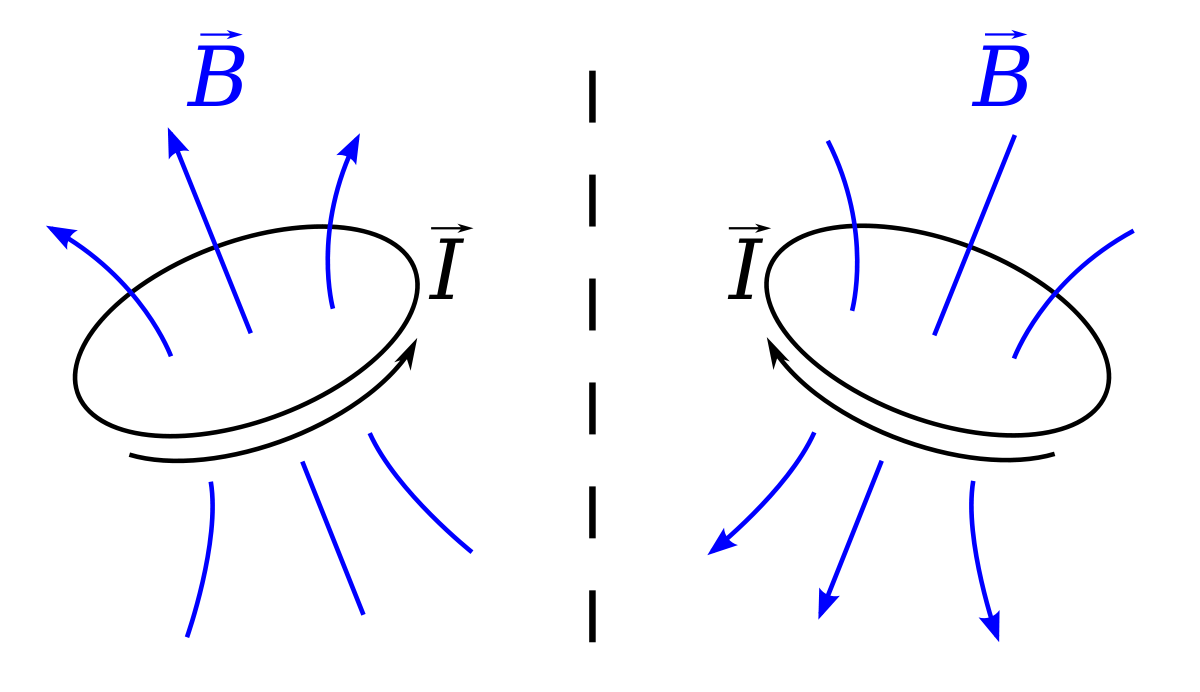
\includegraphics[width=.55\textwidth]{magnetic_field.png}
    \caption{With current flowing in the direction of $\boldsymbol{\vec{I}}$, we see a magnetic field $\boldsymbol{\vec{B}}$ generated from this.  Mirroring the direction of the current flips the magnetic field direction.}
\end{figure}

Said differently, a current loop has a \boldblue{magnetic moment} associated to it. If we have a spinning charged particle with mass $m$, charge $q$, and angular momentum $\vecS$ also has a magnetic moment $\boldsymbol{\vec{\mu}}$ associated to it given by
\[
\boldsymbol{\vec{\mu}} = \frac{g_s q}{2m}\vecS.
\]
If we pass an object with a magnetic moment through an inhomogeneous (nonconstant) magnetic field, it will move in this field. So, if we took a large collection of these particles and shoot them through the same magnetic field, we can observe where these particles end up at. This should tell us about how these particles spin.  In fact, this idea is the exact idea behind the \boldblue{Stern-Gerlach experiment}. There are a few minor differences.

Otto Stern postulated an experiment to look at how atoms spin and Walther Gerlach ran this experiment to test the knownledge of the time.  There, Gerlach placed silver in an oven to create a stream of silver atoms that could be passed through a collimator. The collimator aligns the stream of atoms into a coherent beam that can then be passed through a large magnet with an inhomogeneous magnetic field.  Due to the structure of the silver atom, if it was spinning along the magnetic field we would see the atoms would be deflected from the beam path and a glass plate would measure where the atom then landed. 

\begin{figure}[H]
    \centering
    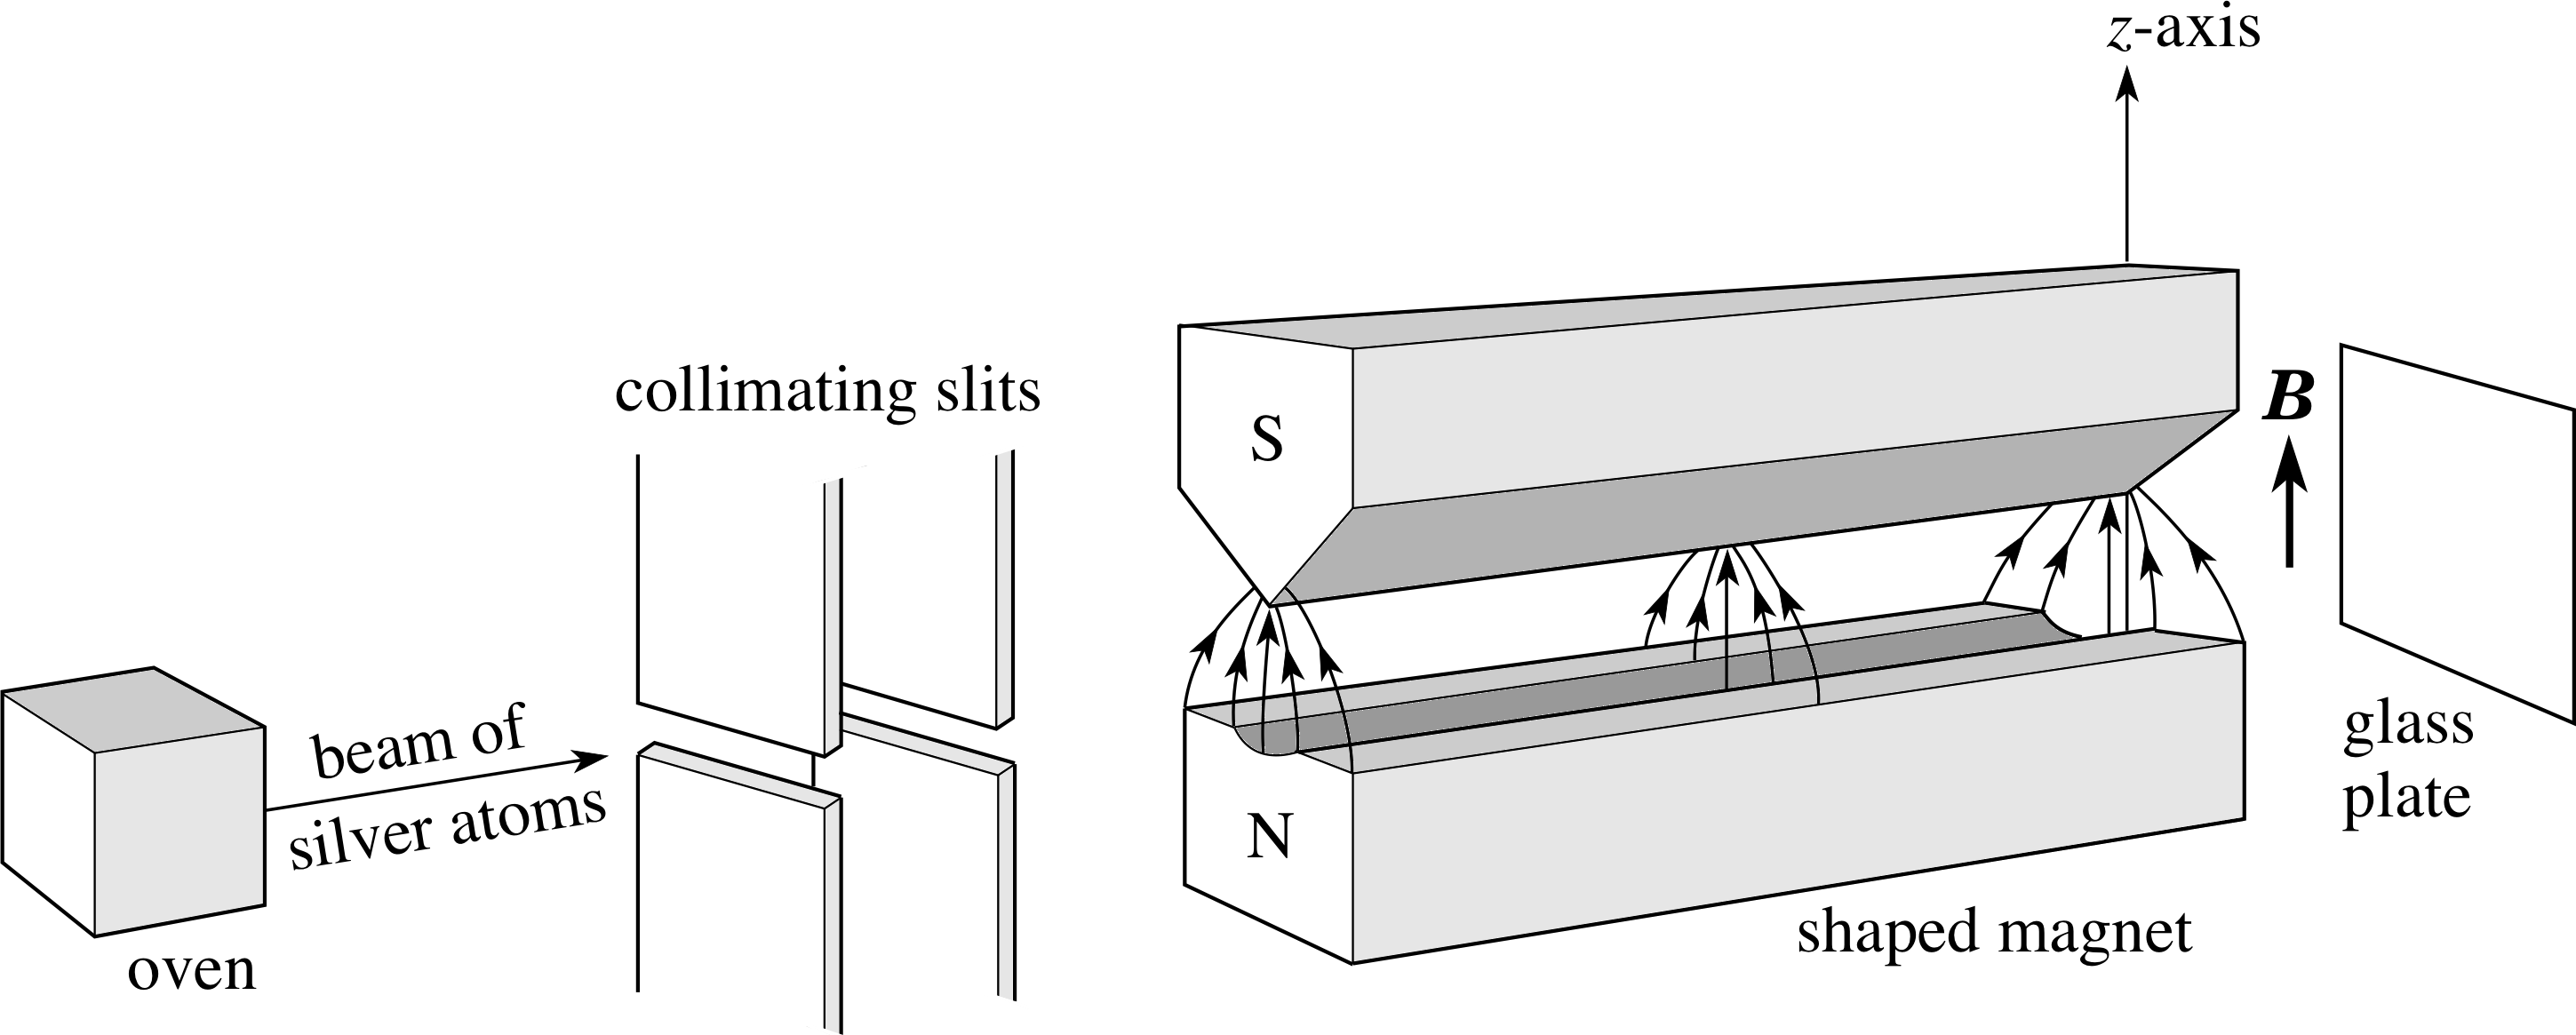
\includegraphics[width=.6\textwidth]{stern_gerlach.png}
    \caption{The experimental set up for Gerlach's experiment.}
\end{figure}

We will refer to this as a \boldblue{Stern-Gerlach apparatus}. Classically, there is no reason to believe that these atoms would prefer spinning in one direction versus another. What was observed was the following.

\begin{figure}[H]
    \centering
    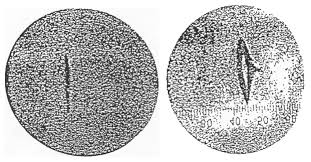
\includegraphics[width=.6\textwidth]{result.jpg}
    \caption{The result of Gerlach's experiment. Left shows the distribution when there was no magnet present and the right shows the result with the magnet present.}
\end{figure}

The result was surprising. What you can see is that there were two distinct directions in which atoms were found to be spinning in rather than a whole continuum of directions! If there were a continuum of directions, you would see the right image would have a more filled in ellipse rather than an ellipse that's missing the interior. What's going on here?

\begin{problem}{Why silver?}{prob:2}
    Read briefly about why Gerlach chose to use silver atoms and do your best to explain that here.
\end{problem}


\section{Behavior of spin 1/2 particles}

The reason why this experiment had this result comes down to how spin is quantized. Sadly, the idea explained before picturing these particles as little loops of current falls short in explaining what we observe. We must do something to explain the phenomon we see, so we now will make an attempt to model this mathematically.

\subsection{Bras and kets}
To start, we can work with electrons. Electrons are charged and are spin 1/2.  Let us say that we align the Stern-Gerlach apparatus so the magnetic field is aligned with the $\zhat$ direction.  Experimentally, Gerlach showed that particles must either have their angular momentum as $\vecS= + \zhat$ or $\vecS=-\zhat$. So, a \boldblue{spin state} $\ket{\Psi}$ for an electron can be written as a superposition of an \boldblue{spin-up state} $\ket{z_+}$ and a \boldblue{spin-down state} $\ket{z_-}$ as
\[
\ket{\Psi} = a_1 \ket{z_+} + a_2 \ket{z_-},
\]
where $a_1,a_2 \in \C$. This notation we use for states is referred to as \boldblue{Dirac bra-ket notation}. A vector $\ket{\Psi}$ is referred to as \boldblue{ket}. In this sense, $\ket{z_+}$ and $\ket{z_-}$ form a basis for the spin state of an electron. In particular, $\ket{\Psi} \in \C^2$ is nothing more than a 2-dimensional complex vector. 

\begin{problem}{Comparing to classical spinning objects}{prob:3}
    For an object rotating in 3 dimensional space we can specify an axis of rotation with a vector $\boldsymbol{\vec{\omega}}\in \R^3$. Explain how a spinning electron is deviating from this notion.
\end{problem}

We can pair a \boldblue{bra} $\bra{\Psi}$ with a ket to do our computations. Given a ket $\ket{\Psi}$ we can create a bra $\bra{\Psi}$ by using the adjoint operator $\dagger$ to get
\[
\bra{\Psi} = \ket{\Psi}^\dagger = a_1^* \ket{z_+}^\dagger + a_2^* \ket{z_-}^\dagger = a_1 \bra{z_+} + a_2 \bra{z_-},
\] 
where we are using $*$ as the complex conjugate. We see that $\bra{z_+}=\ket{z_+}^\dagger$ and $\bra{z_-}=\ket{z_-}^\dagger$.  We then force the relationships
\begin{equation}
\label{eq:relationships}
\bra{z_+} \ket{z_+} = \bra{z_-}\ket{z_-} = 1 \quad \bra{z_-}\ket{z_+} = \bra{z_+}\ket{z_-} = 0.
\end{equation}
In this sense, $\ket{z_+}$ and $\ket{z_-}$ form an orthonormal basis for the spin state of a spin 1/2 particle. Let $\ket{\Psi}$ be as before and let $\ket{\Phi} = c_1 \ket{z_+} + c_2 \ket{z_-}$ then 
\begin{equation}
\label{eq:spin_1_2_inner_product}
\bra{\Phi}\ket{\Psi} = c_1^* a_1 + c_2^* a_2.
\end{equation}
which mimics the hermitian inner product we have seen before for $\C^2$. All states $\ket{\Psi}$ in quantum mechanics must be properly normalized so we require
\[
\bra{\Psi}\ket{\Psi} = 1.
\]

\begin{problem}{Details for $\bra{\Phi}\ket{\Psi}$}{prob:4}
    Let $\ket{\Psi}$ and $\ket{\Phi}$ be as before. Show using Equation \ref{eq:relationships} that Equation \ref{eq:spin_1_2_inner_product} is true.
\end{problem}

We can compute the likelihood that a particle in a given state $\ket{\Psi}$ is observed to be spin up (exiting the top of the Stern-Gerlach apparatus) or spin down (exiting the bottom of the apparatus) in the following way. If we have $\ket{\Psi}=a_1 \ket{z_+} + a_2 \ket{z_-}$ then 
\begin{align}
    \textrm{Probability of spin up} &= a_1 a_1^* = |a_1|^2,\\
    \textrm{Probability of spin down} &= a_2 a_2^* = |a_2|^2.
\end{align}

\begin{problem}{Probabilities}{prob:5}
    For the following states, show that the states are normalized. Then, determine the likelihood that we observe a particle exiting either the top or bottom of the Stern-Gerlach apparatus.
    \begin{enumerate}[(a)]
        \item $\ket{\Psi} = \frac{1}{\sqrt{2}} \ket{z_+} + \frac{1}{\sqrt{2}} \ket{z_-}$.
        \item $\ket{\Phi} = \frac{1}{\sqrt{3}} \ket{z_+} - \frac{\sqrt{2}}{\sqrt{3}} \ket{z_-}$.
    \end{enumerate}
\end{problem}

If we were to set up this experiment ourselves and observe the output of a beam of atoms, then we cannot fully obtain the spin state $\ket{\Psi}$ of the system. To see why this is true, we can show the following.

\begin{problem}{Unitary (phase) invariance}{prob:6}
    As you found in the previous problem, the spin state $\ket{\Psi} = \frac{1}{\sqrt{2}} \ket{z_+} + \frac{1}{\sqrt{2}} \ket{z_-}$ has a 50\% chance to be spin up or down. Show that the modified state
    \[
    \ket{\tilde{\Psi}} = e^{i \theta_1} \frac{1}{\sqrt{2}} \ket{z_+} + e^{i \theta_2} \frac{1}{\sqrt{2}} \ket{z_-},
    \]
    also has a 50\% chance of being spin up or down when measured in the $\zhat$ direction.
\end{problem}

We now see that there are inherent symmetries in quantum spin systems. In particular, if we multiply the components of a spin state by $e^{i \theta}$ (which we call a \boldblue{phase} and this phase is an element of the unitary group $\operatorname{U}(1)$), then we would observe no differences in the output from the Stern-Gerlach apparatus aligned in the $\zhat$ direction. But what if we aligned the apparatus in a different direction?

\subsection{Spin projection operators}

We will find it becomes easiest to think of kets as column vectors and bras as row vectors. This allows us to work with all of this concretely as matrices. Specifically, we can take
\[
\ket{z_+} = \begin{pmatrix} 1 \\ 0 \end{pmatrix} \qquad \textrm{and} \qquad \ket{z_-}=\begin{pmatrix} 0 \\ 1 \end{pmatrix}.
\]
Then we have
\[
\ket{\Psi} = \begin{pmatrix} a_1 \\ a_2 \end{pmatrix} \qquad \textrm{and} \qquad \bra{\Psi} = \begin{pmatrix} a_1^* & a_2^* \end{pmatrix}.
\]
Then we can note
\[
\bra{\Phi}\ket{\Psi} = \begin{pmatrix} c_1^* & c_2^* \end{pmatrix} \begin{pmatrix} a_1 \\ a_2 \end{pmatrix} = c_1^*a_1 + c_2^* a_2.
\]

In this same vein, the Stern-Gerlach apparatus aligned in the $\zhat$ direction becomes a linear transformation written as the matrix
\[
S_z = \frac{\hbar}{2} \begin{pmatrix} 1 & 0 \\ 0 & -1 \end{pmatrix},
\]
which we refer to as the \boldblue{spin projection operator}.  This operator is an example of an \boldblue{observable} which is a quantity of a system we can measure and one should think of observables in quantum mechanics as such. Here $\hbar$ is \boldblue{Plank's reduced constant} that has units of angular momentum (which is the same as $\vecS$). As it turns out, the vectors $\ket{+}$ and $\ket{-}$ are eigenvectors of this matrix.

\begin{problem}{Spin eigenstates}{prob:7}
    Find the eigenvalues and show that the eigenvectors are $\ket{z_+}$ and $\ket{z_-}$ for $S_z$. 
\end{problem}

If we then took a new Stern-Gerlach apparatus oriented along the $\xhat$ direction, we would get the spin projection operator
\[
S_x = \frac{\hbar}{2} \begin{pmatrix} 0 & 1 \\ 1 & 0 \end{pmatrix}
\]
and if we had another oriented in the $\yhat$ direction, we have the spin projection operator
\[
S_y = \frac{\hbar}{2} \begin{pmatrix} 0 & -i \\ i & 0 \end{pmatrix}.
\]

\begin{problem}{Spin projection operators are hermitian}{prob:6}
    Show that the matrices $S_x$, $S_y$, and $S_z$ are hermitian. What does this tell us about the eigenvectors and eigenvalues of these matrices?
\end{problem}

\begin{problem}{Eigenvectors for other spin projection operators}{prob:8}
    \begin{enumerate}[(a)]
        \item Show that the eigenvalues of $S_x$ and $S_y$ are also $\pm\frac{\hbar}{2}$.
        \item Show that the corresponding normalized eigenvectors of $S_x$ are
        \[
        \ket{x_+} = \frac{1}{\sqrt{2}} \begin{pmatrix} 1 \\ 1 \end{pmatrix} \qquad \textrm{and} \qquad \ket{x_-} = \frac{1}{\sqrt{2}} \begin{pmatrix} 1 \\ -1 \end{pmatrix}.
        \]
        \item Show that $\ket{x_+}$ and $\ket{x_-}$ are orthogonal.
        \item Show that the corresponding normalized eigenvectors of $S_y$ are
        \[
        \ket{y_+} = \frac{1}{\sqrt{2}} \begin{pmatrix} 1 \\ i \end{pmatrix} \qquad \textrm{and} \qquad \ket{y_-} = \frac{1}{\sqrt{2}} \begin{pmatrix} 1 \\ -i \end{pmatrix}.
        \]
        \item Show that $\ket{y_+}$ and $\ket{y_-}$ are orthogonal.
    \end{enumerate}
\end{problem}

\subsection{Multiple Stern-Gerlach apparati}

Spin becomes more interesting when we combine together more Stern-Gerlach apparati. Take a look at the following diagram.

\begin{figure}[H]
    \centering
    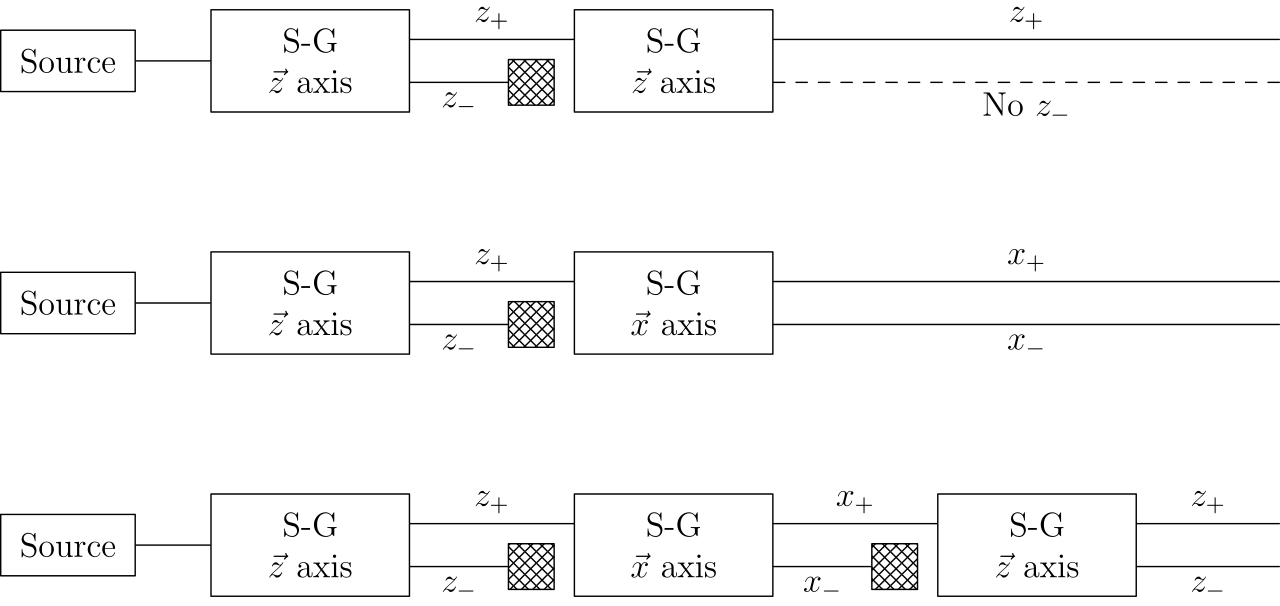
\includegraphics[width=.8\textwidth]{multiple_stern_gerlach.png}
    \caption{A few ways of arranging multiple Stern-Gerlach apparati.}
\end{figure}

First, if we pass a particles through a Stern-Gerlach apparatus oriented in the $\zhat$ direction, we will see two streams of particles exiting; one with spin up particles (e.g., particles with spin state $\ket{\Psi} = \ket{z_+}$ and the other stream will have spin down particles.  If we pass solely spin up particles through another Stern-Gerlach apparatus oriented along the $\zhat$ direction, then we will only observe spin up particles exiting. This is due to the fact that the spin projection operator $S_z$ commutes with itself. We define the \boldblue{commutator bracket} to be
\[
[A,B] = AB-BA.
\]
It is quite clear that we have $[S_z,S_z]=0$ since $S_zS_z-S_zS_z = 0$, where here we take 0 to be the zero matrix.

This commutator bracket  tells us more. Specifically, it tells us when two observables are \boldblue{compatible} with one another.  Here, two observables are said to be compatible if the action of one observation does not influence another. Mathematically, two observables $A$ and $B$ are compatible if $[A,B]=0$. One should recall that matrix multiplication is not always commutative so there can be incompatible observables. 

\begin{problem}{Spin projection observables are not compatible}{prob:9}
\begin{enumerate}[(a)]
    \item Show that $[S_x,S_y]=i\hbar S_z$.
    \item Show that $[S_y,S_z] = i\hbar S_x$.
    \item Show that $[S_z,S_x] = i\hbar S_y$.
\end{enumerate}
\end{problem}

It appears by these calculations that a measurement of spin in one direction and then a new measurement performed after in a different direction will result in incompatibility. We can see this incompatibility in the following example.

Since $[S_z,S_x]\neq 0$, we can consider what happens if we take a stream of particles, pass it through a $\zhat$ oriented Stern-Gerlach apparatus, and then measure the particles that exit in the state $\ket{z_+}$ with another Stern-Gerlach apparatus aligned in the $\xhat$ direction. Thus, we need to write $\ket{z_+}$ in terms of the $x$ spin up state $\ket{x_+}$ and the $x$ spin down state $\ket{x_-}$ as
\[
\ket{z_+} = a_1 \ket{x_+} + a_2 \ket{x_-}.
\]

\begin{problem}{Probability of spin in a different direction}{prob:10}
    To determine the constants $a_1$ and $a_2$ above, we can project $\ket{z_+}$ onto the $x$ spin basis. So, we can take
    \[
        a_1 = \bra{z_+}\ket{x_+} \qquad \textrm{and} \qquad a_2 = \bra{z_+}\ket{x_-}.
    \]
    What is the likelihood that a particle prepared in the state $\ket{z_+}$ will exit a Stern-Gerlach apparatus oriented along the $\xhat$ direction with spin up or spin down? 

    Repeat this process for the $z$ spin down state $\ket{z_-}$.
\end{problem}

In the previous problem, one should then observe that we will see an equal likelihood of seeing spin up or spin down in the $\xhat$ direction once the particles exit the first $\zhat$ oriented Stern-Gerlach apparatus. These two distinct measurements are incompatible with one another. If we measured the $\xhat$ spin first, we may see a different likelihood to see particles as $x$ spin up or $x$ spin down but if we pass it through a $\zhat$ oriented apparatus first, the outcome of a subsequent $\xhat$ spin measurement will always yield 50\% spin up and 50\% spin down. 

\begin{remark}
    This all goes to show that one cannot entirely determine the spin state of a single particle. For example, one would have to first observe the $\zhat$ spin then the $\xhat$ spin, but the act of performing the $\zhat$ measurement before the $\xhat$ measurement destroys the $\xhat$ spin information!
\end{remark}

Finally, if we first pass a particle through an $\zhat$ oriented apparatus, second a $\xhat$, third a $\zhat$ apparatus again, one might expect that we should already know the $\zhat$ spin information. For example, in Figure 5, we take the spin up output of the $\zhat$ apparatus and pass it through the $\xhat$. From there, we take the $x$ spin up particles and pass them through another $\zhat$ apparatus an observe two streams even though our particles were at one point in time measured as $z$ spin up. Let's see this mathematically.

\begin{problem}{Three apparati}{prob:11}
    In the previous problem, you found that you can write $\ket{z_+}$ in terms of $\ket{x_+}$ and $\ket{x_-}$.  If we take a stream of particles in state $\ket{x_+}$, we can then see how this state is composed of $\ket{z_+}$ and $\ket{z_-}$ states.

    Write $\ket{x_+}$ in terms of $\ket{z_+}$ and $\ket{z_-}$ and argue why we will see equal amounts of $z$ spin up particles leave the third apparatus despite the fact that all of these particles were previously in state $\ket{z_+}$.
\end{problem}

\begin{remark}
    The above result now explicitly shows that our incompatible observables destroy information. Though we knew a particle was in a $\ket{z_+}$ state, by passing it through a $\zhat$ oriented apparatus we then find the $z$ spin information is destroyed.
\end{remark}


\section{Entanglement}

Finally, let us discuss what it means for two spin 1/2 particles to be entangled. The mathematics behind this concept lead to a clear understanding of what happens (contrary to some pop. sci. articles).  If we have two spin 1/2 particles in states $\ket{\Psi_1}$ and $\ket{\Psi_2}$ (the subscripts label the particle number) we can form a composite state $\ket{\Psi}$ for both particles.

In the broadest generality, a state of the composite system (for both particles at once) is given by a linear combination 
\[
\ket{\Psi} = a_1 \ket{z_+} \otimes \ket{z_+} + a_2 \ket{z_+} \otimes \ket{z_-} + a_3 \ket{z_-} \otimes \ket{z_+} + a_4 \ket{z_-} \otimes \ket{z_-}.
\]
The symbol $\otimes$ is formal notation allowing us to combine together two vectors into a new object that one can call a \boldblue{tensor}.  We will not discuss tensors abstractly, but one should imagine that this is just a way of combining two vector spaces (and thus the vectors in those spaces) together. New notation aside, the interpretation of the above linear combination can be interpreted quite simply. In particular,
\begin{align}
    \textrm{Probability of particle 1 spin up and particle 2 spin up} &= a_1 a_1^* = |a_1|^2,\\
    \textrm{Probability of particle 1 spin up and particle 2 spin down} &= a_1 a_1^* = |a_2|^2,\\
    \textrm{Probability of particle 1 spin down and particle 2 spin up} &= a_1 a_1^* = |a_3|^2,\\
    \textrm{Probability of particle 1 spin down and particle 2 spin down} &= a_1 a_1^* = |a_1|^2.
\end{align}

Now, if we have
\[
\ket{\Psi_1} = a_{11} \ket{z_+} + a_{12} \ket{z_-} \qquad \textrm{and} \qquad \ket{\Psi_2} = a_{21} \ket{z_+} + a_{22} \ket{z_-},
\]
we can create a state by doing the following
\begin{align*}
\ket{\Psi_1}\otimes \ket{\Psi_2} &=  (a_{11} \ket{z_+} + a_{12} \ket{z_-}) \otimes (a_{21} \ket{z_+} + a_{22} \ket{z_-})\\
&= a_{11}a_{21} \ket{z_+} \otimes \ket{z_+} + a_{11} a_{22} \ket{z_+} \otimes \ket{z_-} + a_{12} a_{21} \ket{z_-} \otimes \ket{z_+} + a_{12}a_{22} \ket{z_-} \otimes \ket{z_-}.
\end{align*}
If the composite state for the system $\ket{\Psi}$ is given by 
\begin{equation}
\label{eq:entangled_state}
\ket{\Psi} = \ket{\Psi_1} \otimes \ket{\Psi_2},
\end{equation}
then we say that this is a \boldblue{separable} state of the system. However, if we \textbf{cannot} write $\ket{\Psi} = \ket{\Psi_1} \otimes \ket{\Psi_2}$ then we say two particles are \boldblue{entangled}.  

It is now time to introduce the most famous couple in science, Alice and Bob.  Alice and Bob work together on many team assignments, and now their task is as follows: breakdown a state of a composite system to see if it is entangled or not. Both of these scientists enjoy experiments and theory, so they're going to work on both sides of the story.

\begin{problem}{An entangled state}{prob:12}
Consider the state of a composite system
\[
\ket{\Psi} = \frac{1}{\sqrt{2}} ( \ket{z_-} \otimes \ket{z_+} - \ket{z_+} \otimes \ket{z_-}).
\]
\begin{enumerate}[(a)]
    \item The two particles are prepared in the state $\ket{\Psi}$ above and Alice observes particle 1 to be spin up. If Bob measures particle 2, what must the spin of that particle be?
    \item Show that we cannot write $\ket{\Psi}=\ket{\Psi_1}\otimes \ket{\Psi_2}$ for any states $\ket{\Psi_1}$ and $\ket{\Psi_2}$.
\end{enumerate}
\end{problem}

\begin{problem}{An non-entangled state}{prob:13}
Consider the state of a composite system
\[
\ket{\Psi} = \frac{1}{2} ( \ket{z_+} \otimes \ket{z_+} - \ket{z_+} \otimes \ket{z_-} + \ket{z_-}\otimes \ket{z_+}-\ket{z_-}\otimes \ket{z_-}).
\]
\begin{enumerate}[(a)]
    \item The two particles are prepared in the state $\ket{\Psi}$ above and Alice observes particle 1 to be spin up. What is the likelihood that Bob sees his particle as spin up?
    \item Show that $\ket{\Psi}=\ket{\Psi_1}\otimes \ket{\Psi_2}$ for some states $\ket{\Psi_1}$ and $\ket{\Psi_2}$.
\end{enumerate}
\end{problem}

\section{Conclusion}

    This brief foray into spin should provide you some more context on why we develop mathematics with complex vector spaces, inner products, and adjoints.  It should also motivate further topics such as tensors. The story here is also incomplete. Particles do not have to just be spin 1/2, they can exist in spin spates $n/2$ for any $n=1,2,3,\dots$.  For example, a photon is a spin 1 particle.  These higher spin particles simply exist in higher dimensional complex vector spaces. For spin 1/2 we saw there can be spin up or down, but in the spin 1 case, we can observe spin up, spin down, and no spin. Observables and operators motivate a large amount of our future endeavors. In fact, there is a whole field of mathematics devoted to the study of operators. Largely, this was motivated by quantum mechanics. 

    One could go on to talk about fermions and bosons. That is, particles with half integer spin (1/2, 3/2, 5/2, ...) and integer spin (1,2,3,...) respectfully. These particles interact differently. Fermions are repulsed by one another whereas bosons are attracted to one another. Those properties in particular lead to the Pauli exclusion principle and Bose-Einstein condensates.  All interesting, but require quite a bit more work.

    At any rate, you have now gotten a cursory glance into more quantum mechanics. Specifically, the place where states of the quantum system are finite dimensional. We have studied the particle in a box as well as the quantum harmonic oscillator before, and those states (believe it or not) live in an infinite dimensional vector space. Perhaps that is why some authors choose to start with spin systems.

    We will move on to work with functions in higher dimensions and differential equations with these functions. This will lead us into deepening our understanding of linear algebra enough to think of these types of equations in terms of linear algebra -- just with infinite dimensions. Moreover, this will lead us to some wonderful results like the Fourier series and transform. Stay tuned!
\end{document}
